\section{APX-completeness for segments parallel to axes}
\label{section:segment_apx}

In this section we analyze whether there exists 
PTAS for geometric set cover for rectangles.
We show that we can restrict this problem
to a very simple setting:
segments parallel to axes and allow (1/2)-extension,
and the problem is still APX-hard.
Note that segments are just degenerated rectangles
with one side being very narrow.


Our results can be summarized in the following
theorem and this section aims to prove it.

\begin{tw}{
\label{segment_cover_apx_hard}
	\textbf{(axis-parallel segment set cover with 1/2-extension is APX-hard)}.	
	Unweighted geometric set cover
	with axis-parallel segments in 2D (even with 1/2-extension)
	is APX-hard.
	That is, assuming $P\neq NP$, there does not exist a PTAS
	for this problem.
}\end{tw}
 
Theorem \ref{segment_cover_apx_hard} implies the following.

\begin{corollary}{
\label{rectangle_cover_apx_hard}
	\textbf{(rectangle set cover is APX-hard)}.	
	Unweighted geometric set cover
	with rectangles (even with 1/2-extension) is APX-hard.
}\end{corollary}


We prove Theorem \ref{segment_cover_apx_hard}
by taking a problem that is APX-hard
and showing a reduction.
For this problem we choose
MAX-(3,3)-SAT which we define below.


\subsection{MAX-(3,3)-SAT and statement of reduction}
\begin{defi}
\textbf{MAX-3SAT} is the following maximization problem. We are given a 3-CNF
formula, and need to find an assignment of variables
that satisfies the most clauses.
\end{defi}

\begin{defi}
\textbf{MAX-(3,3)-SAT} is a variant of MAX-3SAT with an additional
restriction that every variable appears in exactly 3 clauses.
Note that thus, the number of clauses is equal to the number of variables.
\end{defi}

In our proof of Theorem \ref{segment_cover_apx_hard} we use
hardness of approximation of MAX-(3,3)-SAT proved
in \cite{hastad} and described in
Theorem \ref{hastadtheorem} below.

\begin{defi}[$\alpha$-satisfiable MAX-3SAT formula]
MAX-3SAT formula of size $n$ is at most $\alpha$-satisfiable, if
every assignment of variables does not satisfy more than $\alpha n$
clauses. 
\end{defi}

\begin{tw}{
	\label{hastadtheorem}
	\textbf{\cite{hastad}}
	
	For any $\epsilon > 0$, it is NP-hard to distinguish satisfiable
	(3,3)-SAT formulas from
	%This broke x-satisfiable to next line
	at most
	\linebreak\mbox{$(7/8 + \epsilon)$-satisfiable}
	(3,3)-SAT formulas.
}\end{tw}


Given an instance $I$ of MAX-(3,3)-SAT,
we construct an instance $J$ of 
axis-parallel segment set cover problem,
such that for a sufficiently small $\epsilon > 0$,
a polynomial time $(1+\epsilon)$-approximation algorithm for $J$
would be able to distinguish  whether an instance $I$ of MAX-(3,3)-SAT
is fully satisfiable
or is at most $(7/8 + \epsilon)$-satisfiable.
However, according to (Theorem \ref{hastadtheorem}) the latter problem
is NP-hard.
That would imply P = NP, contradicting the assumption.

The following lemma encapsulates the properties
of the reduction described in this section,
and it allows us to prove Theorem \ref{segment_cover_apx_hard}.

\begin{lemma}{
	\label{apxconstruction}
	Given an instance $S$ of  MAX-(3,3)-SAT 
	with $n$ variables and optimum value $opt(S)$,
	we can construct an instance $I$ of geometric set cover with
	axis-parallel segments in 2D, such that:
	\begin{enumerate}[label={(\arabic*)}]
	\item For every solution $X$ of instance $I$,
	there exists a solution of $S$ that satisfies at least  $15n - |X|$
	clauses.
	
	\item For every solution of instance $S$ that satisfies $w$ clauses,
	there exists a solution of $I$ of size $15n - w$.
	
	\item Every solution with $1/2$-extensions of $I$
	is also a solution to the original instance $I$.
		
	Therefore, the optimum size of a solution of $I$
	is $opt(I) = 15n - opt(S)$. 
	\end{enumerate}
	
}\end{lemma}

We prove Lemma \ref{apxconstruction} in
subsequent sections, but meanwhile let us prove
Theorem \ref{segment_cover_apx_hard} using Lemma \ref{apxconstruction}
and Theorem \ref{hastadtheorem}.

TODO: This below can't use current template

\begin{proof}[Proof of Theorem \ref{segment_cover_apx_hard}].
Consider any $0 < \epsilon < 1/(15 \cdot 8)$.

Let us assume that there exists a polynomial-time
$(1+\epsilon)$-approximation algorithm
for unweighted geometric set cover with axis-parallel segments in 2D
with (1/2)-extensions.
We construct an algorithm that solves the problem stated in 
Theorem \ref{hastadtheorem}, thereby proving that P = NP.

Take an instance~$S$ of MAX-(3,3)-SAT to be distinguished
and construct an instance of geometric set cover $I$
using Lemma \ref{apxconstruction}.
We now use the $(1+\epsilon)$-approximation algorithm
for geometric set cover on $I$.
Denote the size of the solution returned by this algorithm as $approx(I)$.
We prove that 
if in $S$
one can satisfy at most $(\frac{7}{8}+\epsilon)n$ clauses,
then $approx(I) \ge 15n - (\frac{7}{8} + \epsilon)n$
and if $S$ is
satisfiable, then $approx(I) < 15n - (\frac{7}{8} + \epsilon)n$.

\subparagraph{Assume $S$ satisfiable.}
From the definition of $S$ being satisfiable, we have:
$$opt(S) = n.$$

From Lemma \ref{apxconstruction} we have:

$$opt(I) = 14n.$$

Therefore,
$$approx(I) \le (1+\epsilon)opt(I) = 14n(1+\epsilon)
	= 14n + 14\epsilon\cdot n =$$ 
	$$= 14n + (15\epsilon - \epsilon)n < 
  14n + \left(\frac{1}{8} - \epsilon\right)n 
= 15n - \left(\frac{7}{8} + \epsilon\right)n$$

\subparagraph{Assume $S$ is at most 
$\left(\frac{7}{8} + \epsilon\right)$ satisfiable.}
From the defintion of $S$ being at most 
$\left(\frac{7}{8} + \epsilon\right)n$ satisfiable, we have:
$$opt(S) \le \left(\frac{7}{8} + \epsilon\right)n$$

From Lemma \ref{apxconstruction} we have:
$$opt(I) \ge 15n - \left(\frac{7}{8} + \epsilon\right)n$$

Since a solution to $I$ with $\frac{1}{2}$-extensions is
also a solution without extentions, by 
Lemma \ref{apxconstruction} (3.), we have:

$$approx(I) \ge opt(I) = 15n - \left(\frac{7}{8} + \epsilon\right)n$$


Therefore, by using the assumed $(1+\epsilon)$-approximation
algorithm,
it is possible to distinguish the case when
$S$ is satisfiable from the case when it is
at most $(\frac{7}{8} + \epsilon)n$ satisfiable,
it suffices to compute $approx(I)$ with $15n - (\frac{7}{8}+\epsilon)n$.
Hence, the assumed approximation algorithm cannot exist, unless P = NP.

\end{proof}

\subsection{Reduction construction}
We show reduction from MAX-(3,3)-SAT problem
to geometric set cover with segments
parallel to axis. Moreover the instance
of geometric set cover will be robust
to 1/2-extensions (have the same optimal solution
after 1/2-extension).

The construction will be composed of 2 types of gadgets:
\textbf{VARIABLE-gadgets} and \textbf{CLAUSE-gadgets}.
CLAUSE-gadgets would be constructed using two \textbf{OR-gadgets}
connected together.


\subsubsection{VARIABLE-gadget}

VARIABLE-gadget is responsible for choosing the value of a variable
in a CNF formula. It allows two minimal solutions
and every minimal solution must use exactly one of the
$\xTrueSegment$ and $\xFalseSegment$
segments. These two choices correspond to the two Boolean values of the variable.

\paragraph{Points.}

Define points:
\begin{figure}[h]
\centering
\def\svgwidth{0.5\columnwidth}
\input{apx_choose_variable.pdf_tex}
\caption{\textbf{VARIABLE-gadget.}
We denote the set of points marked with black circles as $C_{var}^i$,
and they need to be covered (are part of the set $\points$).
Note that some of the points are not marked as black dots
and exists only to name segments for further reference.
We denote the set of red segments as $X_{false}^i$
and the set of green segments as $X_{true}^i$.}
\label{fig:apx_choose_variable}
\end{figure}

With $L = 12n$:

\begin{center}
\begin{tabular}{ l l l l}
	$a = (-L, 0)$ &
	$b = (-\frac{2}{3}L, 0)$ & 
	$c = (-\frac{1}{3}L, 0)$ & 
	$d = (-L, 1)$ \\  
	$e = (-\frac{2}{3}L, 1)$ & 
	$f = (-\frac{2}{3}L, 2)$ &
	$g = (L, 0)$ &
	$h = (L, 2)$
\end{tabular}
\end{center}

Let us define: $$C_{var} =  \{a, b, c, d, e, f\}$$
and $$C_{var}^i = C_{var} + (0, 4i)$$


\paragraph{Segments.}

Let us define:

$$X_{true}^i =\{ (a_i, d_i), (b_i, f_i), (c_i, g_i)\}$$
$$X_{false}^i = \{(a_i, c_i), (d_i, e_i), (f_i, h_i)\}$$

$$P_{var}^i = X_{true}^i \cup X_{false}^i$$


\begin{lemma}
\label{choose_variables_solution}
For any $1 \le i \le n$, points $C_{var}^i$
can be covered using 3 segments from $P_{var}^i$.
\end{lemma}

\begin{proof}
We can use either set $X_{true}^i$ or $X_{false}^i$.
\end{proof}

\begin{lemma}
\label{choose_variables_no_less}
For any $1 \le i \le n$, points $C_{var}^i$
can not be covered with less than 3 segments from $P_{var}^i$.
\end{lemma}

\begin{proof}
No segment of $P_{var}^i$ covers more than one point from
$\{d_i, f_i, c_i\}$, therefore $C_{var}^i$ can
not be covered with less than 3 segments.
\end{proof}

\begin{lemma}
\label{choose_variables_both}
If both segments $\xTrueSegment$ and $\xFalseSegment$ are chosen, then
the covering the remaining points from $C_{var}^i$
requires at least 2 different
segments from $P_{var}^i$.
\end{lemma}
\begin{proof}
No segment of $P_{var}^i$ covers more than one point from
$\{a_i, e_i\}$,
therefore 
$C_{var}^i$ - $\{c_i, f_i, g_i, h_i\}$
can not be covered with less than 2 segments.
\end{proof}


\subsubsection{OR-gadget}

OR-gadget has 3 important segments
-- $x, y, result$. $x$ and $y$ don't count to the weight of solution
of OR-gadget (they are part of different gadgets).
It has a minimal solution of weight $w$
and $result$ can be chosen only if $x$ or $y$ are also chosen
for the solution.
If none of them are chosen, then solution
choosing $result$ segment has weight at least $w+1$.
Therefore the following formula holds for a solution $R$
assuming that $R$ uses only $w$ from this OR-gadget:

$$ (x \in R) \lor (y \in R) \iff result \in R  $$

\paragraph{Points.}

\begin{figure}[h]
\centering
\def\svgwidth{0.5\columnwidth}
\input{apx_or_gadget.pdf_tex}
\caption{
\textbf{OR-gadget.} We denote these point as $or\_gadget_{i, j}$. 
We denote set of red segments as $or^{false}_{i, j}$,
set of blue segments as $or^{true}_{i, j}$,
green and yellow segments as $or\_move\_variable_{i, j}$.
}
\label{fig:apx_or_gadget}
\end{figure}

	\begin{center}
\begin{tabular}{ l l l l}

	$l_0 = (0, 0)$ &
	$m_0 = (0, 1)$ &
	$n_0 = (0, 2)$ &
	$o_0 = (0, 3)$ \\
	$p_0 = (0, 4)$ &
	$q_0 = (1, 1)$ &
	$r_0 = (1, 3)$ &
	$s_0 = (2, 1)$ \\
	$t_0 = (2, 2)$ &
	$u_0 = (2, 3)$ &
	$v_0 = (3, 2)$ &
\end{tabular}
\end{center}


	$$vec_{i, j} = (10i + 3 + 3j, 4n + 2j)$$
	
	Define 
	$\{ l_{i, j}, m_{i, j} \ldots v_{i, j} \}$
	as $\{l_0, m_0 \ldots v_0\}$ shifted by $vec_{i, j}$

Note that $v_{i, 0} = l_{i, 1}$ (see Figure~\ref{fig:apx_clause})
 
  $$C\_or\_gadget_{i, j} = 
 \{l_{i, j}, m_{i, j}, n_{i, j}, o_{i, j},
 p_{i, j}, q_{i, j}, r_{i, j}, s_{i, j}, t_{i, j}, u_{i, j} \}
 $$
 
\paragraph{Segments.}

We define names subsets of segments, to refer to them in lemmas.
 
$$or^{false}_{i, j} =
\{ (q_{i, j}, r_{i, j}), (s_{i, j}, u_{i, j})\}$$
$$or^{true}_{i, j} =
\{ (m_{i, j}, s_{i, j}), (o_{i, j}, u_{i, j}),
(t_{i, j}, v_{i, j}) \}$$

$$or\_move\_variable_{i, j} =
\{ (l_{i, j}, n_{i, j}), (n_{i, j}, p_{i, j})\}$$

Segments in OR-gadget:

$$P\_or\_gadget_{i, j} = 
  or^{false}_{i, j} \cup or^{true}_{i, j} \cup or\_move\_variable_{i, j}
  $$


\begin{lemma}
\label{cover_or_true}
For any $1 \le i \le n, j \in \{0, 1\}$ and 
 $x \in \{l_{i, j}, p_{i, j}\}$ we can cover points in
$C\_or\_gadget_{i, j} - \{ x\} \cup \{v_{i, j}\}$
with 4 segments.
\end{lemma}

\begin{proof}
We can do that using one segment from
$or\_move\_variable_{i, j}$
(chosen depending on the value of $x$)
and all segments from $or^{true}_{i, j}$.
\end{proof}

\begin{lemma}
\label{cover_or_false}
For any $1 \le i \le n, j \in \{0, 1\}$, we can cover points in
$C\_or\_gadget_{i, j}$ with 4 segments from $P\_or\_gadget_{i,j}$.
\end{lemma}

\begin{proof}
We can do that using  $or\_move\_variable_{i, j}$
and $or^{false}_{i, j}$.
\end{proof}


\subsubsection{CLAUSE-gadget}


CLAUSE-gadget is responsible for calculating if choice of the
variable values meets the clause in formula.
It has minimal solution of weight $w$ if at least one variable
in the clause has a correct value.
Otherwise it has minimal solution $w+1$.
This way by the minimal solution for the whole problem, we can tell
how many clauses were satisfiable.

The CLAUSE-gadgets consist of two OR-gadgets.
We don't want the CLAUSE-gadgets to be crammed 
somewhere between
the very long variable segments. That's why we have a simple
gadget to \textit{pass} the value of the segment, ie. segments
$(x_{i, 0}, x_{i, 1}), (y_{i, 0}, y_{i, 1}), (z_{i, 0}, z_{i, 1})$.
Two segments and one of them is chosen if $x$ was chosen
in the solution and the other one if $x$ wasn't.

\paragraph{Points.}


\begin{figure}[h]
\centering
\def\svgwidth{0.8\columnwidth}
\input{apx_clause.pdf_tex}
\caption{\textbf{CLAUSE-gadget.}
We denote set of these points as $C\_clause_i$.
Every green rectangle is an OR-gadget.
$y$-coordinates of $x_{i, 0}$, $y_{i, 0}$ and $z_{i,0}$
depend on the values of variables in the $i$-th clause.
}
\label{fig:apx_clause}
\end{figure}

TODO: Rephrase it

Assuming clause $C_i = x_i \lor y_i \lor z_i$,
function $idx(w)$ is returning index of the variable $w$,
function $neg(w)$ is returning whether variable $w$ is negated
in a clause.

\begin{center}
\begin{tabular}{ l l }
	$x_{i, 0} = (10i+1, 4\cdot idx(x_i) + 2\cdot neg(x_i))$ &
	$x_{i, 1} = (10i+1, 4n)$ \\
	$y_{i, 0} = (10i+2, 4\cdot idx(y_i) + 2\cdot neg(y_i))$ &
	$y_{i, 1} = (10i+2, 4n + 4)$ \\
	$z_{i, 0} = (10i+3, 4\cdot idx(z_i) + 2\cdot neg(z_i))$ &
	$z_{i, 1} = (10i+3, 4n + 6)$
\end{tabular}
\end{center}
	
 
 $$move\_variable_i = 
 \{x_{i, j} : j \in \{0, 1\}\} \cup
 \{y_{i, j} : j \in \{0, 1\}\} \cup
 \{z_{i, j} : j \in \{0, 1\}\} 
 $$
 
 $$C\_clause_i = 
 move\_variable_i \cup C\_or\_gadget_{i, 0}
 \cup C\_or\_gadget_{i, 1} \cup \{v_{i, 1} \} 
 $$

\paragraph{Segments.}

\begin{eqnarray*}
P\_clause_i & = & \{ (x_{i, 0}, x_{i, 1}),
(y_{i, 0}, y_{i, 1}),
(z_{i, 0}, z_{i, 1}),
(x_{i, 1}, l_{i, 0}),
(y_{i, 1}, p_{i, 0}),
(z_{i, 1}, p_{i, 1}),
\} \cup \\
& & \cup \ P\_or\_gadget_{i, 0} \cup P\_or\_gadget_{i, 1}
\end{eqnarray*}

\begin{lemma}
\label{cover_clauses_solution_true}
For any $1 \le i \le n$ and $a \in \{ x_{i, 0}, y_{i, 0}, z_{i, 0}\}$,
points $C\_clause_i - \{a\}$ can be covered using 11 segments
from $P\_clause_i$.
\end{lemma}

\begin{proof}
For $a = x_{i, 0}$ (analogous proof for $y_{i, 0}$):
First we use Lemma~\ref{cover_or_true} twice with excluded $x = l_{i, 0}$ and
$x = l_{i, 1} = v_{i, 0}$,
resulting with 8 segments $or^{true}_{i, 0} \cup or^{true}_{i, 1}$
which cover all required points apart from
$x_{i, 1}, y_{i, 0}, y_{i, 1}, z_{i, 0}, z_{i, 1}, l_{i, 0}$.
We cover those using additional 3 segments:
$\{ (x_{i, 1}, l_{i, 0}), (y_{i, 0}, y_{i, 1}),
(z_{i, 0}, z_{i, 1}) \}$

For $a = z_{0, i}$:
Using Lemma~\ref{cover_or_false} and Lemma~\ref{cover_or_true} with
$x = p_{i, 1}$,
resulting with 8 segments $or^{false}_{i, 0} \cup or^{true}_{i, 1}$
which cover all required points apart from
$x_{i, 0}, x_{i, 1}, y_{i, 0}, y_{i, 1}, z_{i, 1}, p_{i, 1}$.
We cover those using additional 3 segments:
$\{ (x_{i, 0}, x_{i, 1}), (y_{i, 0}, y_{i, 1}),
(z_{i, 1}, p_{i, 1}) \}$.
\end{proof}

\begin{lemma}
\label{cover_clauses_solution_false}
 Points $C\_clause_i$ can be covered with 12 segments from $P\_clause_i$.
\end{lemma}

\begin{proof}
Using Lemma \ref{cover_or_false} twice we can
cover $or\_gadget_{i,0}$ and  $or\_gadget_{i,1}$
with 8 segments.

To cover the remaining points we additionally use:
$\{ (x_{i, 0}, x_{i, 1}), (y_{i, 0}, y_{i, 1}),
(z_{i, 0}, z_{i, 1}), (t_{i, 1}, v_{i, 1}) \}$

\end{proof}

\begin{lemma}
\label{cover_clauses_segments_no_less}
For any $1 \le i \le n$,
points $C\_clause_i - \{ x_{i, 0}, y_{i, 0}, z_{i, 0}\}$
can not be covered using less than 11 segments from $P\_clause_i$.

All points $C\_clause_i$ can not be covered with less than 12 segments
from $P\_clause_i$.
\end{lemma}


\begin{proof}[Proof of no cover with less than 12 segments.]
There is independent set of 12 points in $C\_clause_i \supseteq
\{ x_{i, 0}, y_{i, 0}, z_{i, 0}, l_{i, 0}, p_{i, 0}, q_{i, 0},
u_{i, 0}, v_{i, 0} = l_{i, 1}, p_{i, 1}, q_{i, 1}, u_{i, 1}, v_{i, 1} \}$.
\end{proof}

\begin{proof}[Proof of no cover with less than 11 segments.]

We can choose disjoint sets $X, Y, Z$ such that
$X \cup Y \cup Z \subseteq C\_clause_i - \{x_{i, 0}, y_{i, 0}, z_{i, 0}\}$
and there are no segments covering points from different sets.
And we prove lower bounds for each of these sets.

$$X = \{x_{i, 1}, y_{i, 1}, z_{i, 1}\}$$

Set $X$ is an indendent set, so it must be covered with 3 segments.

$$Y = or\_gadget_{i, 0} - \{l_{i, 0}, p_{i, 0}\}$$
$$Z = or\_gadget_{i, 1} - \{l_{i, 1}, p_{i, 1}\}$$


For both $Y$ and $Z$ we can check all of the subsets of 3 segments
with brutforce that none of them cover, so they have to be covered with
4 segments.

TODO: Funny fact, neither Y nor Z doesn't have independent set of size 4.

Therefore $C\_clause_i$ must be covered with at least 3 + 4 + 4 = 11 segments.
\end{proof}

\subsubsection{Summary}

Add some smart lemmas that sets will be exclusive to each other.

\begin{lemma}
\textbf{Robustness to 1/2-extensions}. For every segment $s \in \sets$,
$s$ and $s^{+1/2}$ cover the same points from $\points$.
\end{lemma}


\subsection{Summary of contruction}

\begin{figure}
\centering
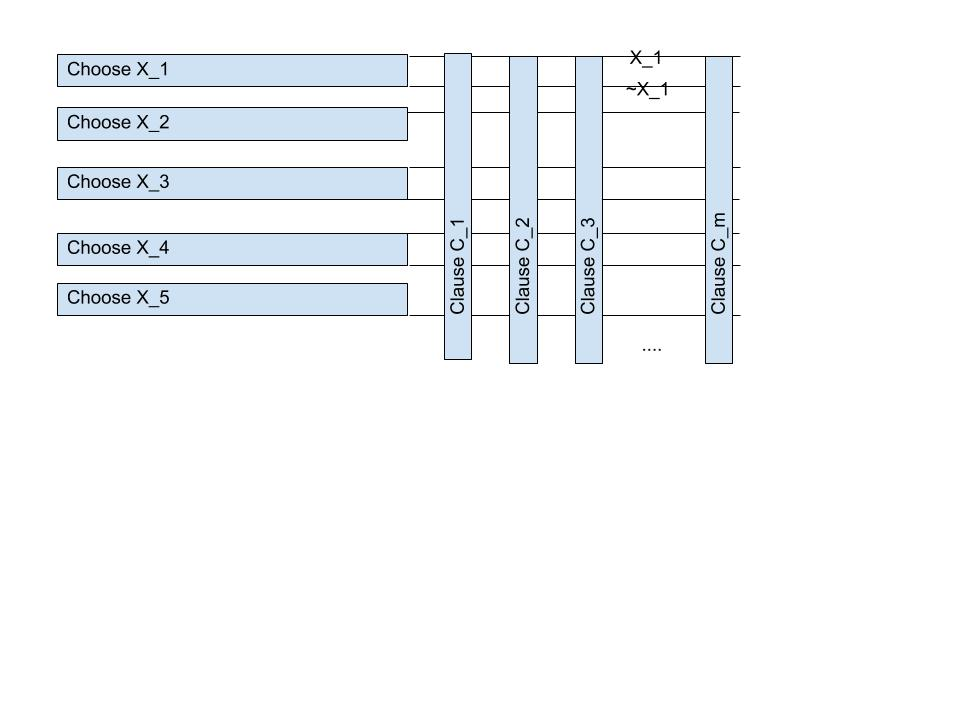
\includegraphics[width=\linewidth]{segment_apx_sketch.jpg}
\caption{\textbf{General schema.}}
General layout of VARIABLE-gadget and CLAUSE-gadget and how they
interact with each other.

TODO: Rename Choose X to VARIABLE-gadget and Clause C to CLAUSE-gadget.
\label{fig:segment_apx_sketch}
\end{figure}

We define:
$$\points := \bigcup_{1 \le i \le n} C\_variable_i \cup C\_clause_i $$
$$\sets := \bigcup_{1 \le i \le n} P\_variable_i \cup P\_clause_i $$

The subsequent sections define these sets.

We prove some properties of different gadgets.
Every segment for a gadget will only cover points 
in this gadget (won't interact with any diferent gadget),
so we can prove lemmas \textit{locally}.


TODO: $y$ axis is increasing values downward on figures
(not upwards like in normal).

\subsection{Proofs of construction Lemma \ref{apxconstruction}}
\begin{lemma}
	\label{construction_correctness}
	Given an instance of MAX-(3,3)-SAT of size $n$
	with optimal solution $k$.
	For instance of geometric cover, constructed
	according to Lemma~\ref{apxconstruction}, 
	there exists a solution of weight $15n - k$.
\end{lemma}

\begin{proof}
Let's name the assignments of the variables in MAX-(3,3)-SAT instance,
that achieve the optimal solution,
$y_1$,~$y_2$~$\ldots$~$y_n$,
Let's cover every VARIABLE-gadget with solution described in
Lemma~\ref{choose_variables_solution},
in the $i$-th gadget choosing the set of segments responsible for the
value of $y_i$
(true -- $x_i^{true}$ or false -- $x_i^{false}$).

Cover every satisfied CLAUSE-gadget with solution described in
Lemma~\ref{cover_clauses_solution_true}
and unsatisfied CLAUSE-gadget with solution from
Lemma~\ref{cover_clauses_solution_false}.

This solution uses $3n + (11m + (m-k)) = 15n - k$ segments.

\end{proof}
\begin{lemma}
	\label{construction_completness}
	Given an instance of MAX-(3,3)-SAT of size $n$,
	and solution of size $w$ to the instance of geometric cover,
	constructed	according to Lemma~\ref{apxconstruction},  
	there exists a solution to MAX-(3,3)-SAT of size at least $15n - w$.
\end{lemma}
\begin{proof}
Among $x_i^{true} \cup x_i^{false}$,
we need to use at least 3 segments (Lemma~\ref{choose_variables_no_less}).
If we have chosen both segments $\xTrueSegment$ and $\xFalseSegment$,
then we have used at least 4 segments (Lemma~\ref{choose_variables_both}).

If we chose at most one of the segments $\xTrueSegment$ and $\xFalseSegment$,
choose the corresponding variable value to the solution.
If we chose both segments,
choose the value that appears in most (at least 2) clauses.
If we have chosen none of the segments, choose any value.

To cover $\bigcup_{1 \le i \le n} C\_variable_i$
we have used at least $3n + a$ segments,
where $a$ is the number of $i$ such that we have chosen both
values $\xTrueSegment$ and $\xFalseSegment$.

Among the segments responsible for the clause $C_i = x \lor y \lor z$
we need to use at least 11 segments
(Lemma~\ref{cover_clauses_segments_no_less})
and if we can cover it with 11 segments, then we have 
earlier chosen
segment responsible for the value of variable $x$, $y$ or $z$
that satisfies $C_i$.

So we have at least 11 segments for satisfied clauses
and at least 12 segments
for unsatisfied clauses, so we cover it with 
at least $11n + b$ segments, where $b$ is number of clauses
where none of the variables $x, y, z$ were chosen.
If the segment responsible for value of $x$ was taken,
but this variable is set to have different value,
then we have chosen segments for both $x$ and $\neg x$ for this variable,
so "we cheated" and this maybe clause is not met,
but we assigned the value for this $x_i$ that meets
the most clauses, so for each of such "cheated" variables,
at most one of the clauses isn't met.

So there are at most $a+b$ unsatsfied clauses in this instance,
so we have shown the assignment with at least  $n-(a+b)$ satisfied clauses.

$$w \ge 3n + a + 11n + b = 14n + a + b$$
$$15n - w  \le 15n - 14 n - a - b = n - (a+b)$$

\end{proof}


\begin{proof}[Proof of Lemma \ref{apxconstruction}]
Given an instance of MAX-(3,3)-SAT of size $n$
with optimal result $k$.
Let's construct an instance of geometric cover,
constructed in aforementioned manner.

Given the Lemma~\ref{construction_correctness}, we know
the optimal solution for the constructed geometric cover is
at most $15n - k$ and since the $k$ is optimal solution
for MAX-(3,3)-SAT, then according to Lemma~\ref{construction_completness}
there doesn't exist a solution with cost less than $15n - k$.
\end{proof}
